% Requires in the preamble:
% \usepackage{amsmath,amssymb}
% \usepackage{tikz,pgfplots}
% \pgfplotsset{compat=1.18}

\chapter{Proofs and Completeness}
\label{app:proofs-completeness}

Most of calculus can be learned first through motion, graphs, rates, and accumulated
area.  But underneath those pictures is a quiet promise:

\[
\boxed{
\text{the limiting objects we are chasing really exist.}
}
\]

A tangent slope is approached by secant slopes.  An integral is approached by Riemann
sums.  A root is trapped by bisection.  A maximum value may be approached by better
and better input choices.

All of those processes need a number line with no holes.

This appendix collects the proof ideas that support that promise.  It is not meant to
replace the main story of the book.  It is a proof workshop: a place to see why the
closed interval \([a,b]\), continuity, and the real numbers are so powerful.

\section{The Least Upper Bound Property}
\label{appsec:least-upper-bound-property}

The real line is more than a long list of numbers.  It has no gaps.

That phrase sounds geometric, but it becomes useful only after we translate it into a
precise statement about sets of numbers.

\subsection{Upper bounds and least upper bounds}
\label{appsubsec:upper-bounds-suprema}

Let \(A\) be a set of real numbers.

A number \(U\) is an \emph{upper bound} for \(A\) if every number in \(A\) is less than
or equal to \(U\):

\[
x\le U
\qquad\text{for every }x\in A.
\]

A set is \emph{bounded above} if it has at least one upper bound.

\paragraph{Example.}
Let

\[
A=(0,1).
\]

Then \(1\) is an upper bound for \(A\), because every \(x\in(0,1)\) satisfies

\[
x\le1.
\]

The number \(2\) is also an upper bound.  So is \(100\).  But \(1\) is the smallest
possible upper bound.

That makes \(1\) the \emph{least upper bound} of \(A\).

\begin{quote}
\textbf{Least upper bound.}
A number \(s\) is the \emph{least upper bound} of a set \(A\) if

\[
\text{1. }s\text{ is an upper bound for }A,
\]

and

\[
\text{2. every upper bound for }A\text{ is at least }s.
\]

The least upper bound is also called the \emph{supremum} of \(A\), written

\[
\boxed{s=\sup A.}
\]
\end{quote}

The supremum does not have to belong to the set.

For

\[
A=(0,1),
\]

we have

\[
\sup A=1,
\]

but

\[
1\notin A.
\]

If the supremum does belong to the set, then it is the maximum.

\paragraph{Example.}
For

\[
B=[0,1],
\]

we have

\[
\sup B=1,
\]

and now

\[
1\in B.
\]

So \(1\) is also the maximum value of \(B\).

\begin{center}
\renewcommand{\arraystretch}{1.5}
\begin{tabular}{c|c|c}
\textbf{set} & \textbf{supremum} & \textbf{maximum?} \\ \hline
\((0,1)\) & \(1\) & no \\
\([0,1]\) & \(1\) & yes \\
\(\{1-\frac1n:n=1,2,3,\ldots\}\) & \(1\) & no \\
\(\{x\in\mathbb R:x^2\le4\}\) & \(2\) & yes
\end{tabular}
\end{center}

The least upper bound is the boundary from above.  A maximum is an element of the
set sitting at that boundary.

\subsection{The completeness axiom}
\label{appsubsec:completeness-axiom}

The real numbers are complete in the following sense.

\begin{quote}
\textbf{Least Upper Bound Property.}
Every nonempty set of real numbers that is bounded above has a least upper bound.
\end{quote}

This is not true for the rational numbers.

Let

\[
A_{\mathbb Q}=\{x\in\mathbb Q:x\ge0\text{ and }x^2<2\}.
\]

This set is nonempty.  For example,

\[
1\in A_{\mathbb Q}.
\]

It is also bounded above.  For example, \(2\) is an upper bound.

Inside the rational numbers, however, there is no rational least upper bound.  The
boundary should be

\[
\sqrt2,
\]

but

\[
\sqrt2\notin\mathbb Q.
\]

The rational line has a hole exactly where the supremum should be.

\begin{figure}[h]
\centering
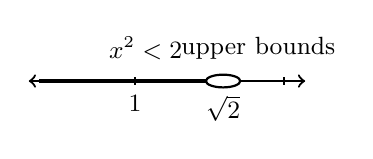
\begin{tikzpicture}[xscale=2.7, every node/.style={font=\small}]
  \draw[<->, thick] (0.5,0) -- (1.8,0);
  \foreach \x/\lab in {1/1,1.414/{\(\sqrt2\)},1.7/{}} {
    \draw[thick] (\x,0.05) -- (\x,-0.05);
  }
  \draw[very thick] (0.55,0) -- (1.414,0);
  \draw[fill=white, thick] (1.414,0) circle (2.3pt);
  \node[below] at (1,-0.06) {\(1\)};
  \node[below] at (1.414,-0.06) {\(\sqrt2\)};
  \node[above] at (1.05,0.15) {\(x^2<2\)};
  \node[above] at (1.58,0.15) {upper bounds};
\end{tikzpicture}
\caption{The set of rational numbers with \(x^2<2\) points toward \(\sqrt2\), which is missing from \(\mathbb Q\).}
\label{fig:rational-hole-sqrt2}
\end{figure}

The real numbers repair this.  In \(\mathbb R\), the same set has a least upper bound,
and that least upper bound is \(\sqrt2\).

\[
\boxed{
\text{Completeness turns limiting boundaries into real numbers.}
}
\]

\subsection{The approximation property of the supremum}
\label{appsubsec:supremum-approximation-property}

The supremum has one small property that is used again and again.

Suppose

\[
s=\sup A.
\]

Then \(s\) is an upper bound.  So every \(a\in A\) satisfies

\[
a\le s.
\]

But \(s\) is the \emph{least} upper bound.  Therefore, if we move even a little below
\(s\), we can no longer have an upper bound.

That gives the following fact.

\begin{quote}
\textbf{Approximation property of the supremum.}
If \(A\) is nonempty and bounded above, and

\[
s=\sup A,
\]

then for every \(\varepsilon>0\), there is an element \(a\in A\) such that

\[
s-\varepsilon<a\le s.
\]
\end{quote}

\paragraph{Proof.}
Since \(s=\sup A\), the number \(s\) is an upper bound for \(A\).  Therefore

\[
a\le s
\]

for every \(a\in A\).

Now let \(\varepsilon>0\).  If no element of \(A\) were larger than \(s-\varepsilon\), then

\[
a\le s-\varepsilon
\]

for every \(a\in A\).  That would make \(s-\varepsilon\) an upper bound for \(A\).

But

\[
s-\varepsilon<s,
\]

contradicting the fact that \(s\) is the least upper bound.

Therefore some \(a\in A\) must satisfy

\[
s-\varepsilon<a.
\]

Together with \(a\le s\), this gives

\[
s-\varepsilon<a\le s.
\]

\begin{quote}
\textbf{Meaning.}
The supremum may not belong to the set, but the set has elements arbitrarily close to
it from below.
\end{quote}

\paragraph{Example.}
Let

\[
A=(0,1).
\]

Then

\[
\sup A=1.
\]

If \(\varepsilon=0.01\), the approximation property says there is an element of \(A\)
between

\[
0.99
\]

and

\[
1.
\]

For example,

\[
0.995\in A.
\]

If \(\varepsilon=10^{-6}\), there is an element of \(A\) between

\[
1-10^{-6}
\]

and

\[
1.
\]

The set never reaches \(1\), but it comes arbitrarily close.

\subsection{Greatest lower bounds}
\label{appsubsec:greatest-lower-bounds}

There is a matching idea from below.

A number \(L\) is a \emph{lower bound} for \(A\) if

\[
L\le x
\qquad\text{for every }x\in A.
\]

A set is \emph{bounded below} if it has a lower bound.

The \emph{greatest lower bound}, or \emph{infimum}, is the largest possible lower
bound.  It is written

\[
\inf A.
\]

\paragraph{Example.}
For

\[
A=(0,1),
\]

we have

\[
\inf A=0.
\]

But \(0\notin A\), so \(A\) has no minimum.

For

\[
B=[0,1],
\]

we have

\[
\inf B=0,
\]

and \(0\in B\), so \(0\) is the minimum.

The Least Upper Bound Property implies the matching lower-bound property: every
nonempty set of real numbers that is bounded below has a greatest lower bound.  One
way to see this is to reflect the set across \(0\).  Lower bounds for \(A\) become upper
bounds for

\[
-A=\{-a:a\in A\}.
\]

So the supremum of \(-A\) gives the infimum of \(A\):

\[
\boxed{
\inf A=-\sup(-A).
}
\]

\section{The Monotone Convergence Theorem}
\label{appsec:monotone-convergence-theorem}

A sequence may wander forever.  But if it moves only in one direction and cannot escape
past a bound, then it must settle down.

That statement is the Monotone Convergence Theorem.

It is one of the first places where completeness does visible work.

\subsection{Monotone sequences}
\label{appsubsec:monotone-sequences}

A sequence

\[
a_1,a_2,a_3,\ldots
\]

is \emph{increasing} if

\[
a_1\le a_2\le a_3\le\cdots.
\]

It is \emph{decreasing} if

\[
a_1\ge a_2\ge a_3\ge\cdots.
\]

A sequence is \emph{monotone} if it is increasing or decreasing.

\paragraph{Example.}
The sequence

\[
a_n=1-\frac1n
\]

is increasing:

\[
0,\ \frac12,\ \frac23,\ \frac34,\ldots.
\]

It is bounded above by \(1\).  The terms approach \(1\).

\paragraph{Example.}
The sequence

\[
b_n=\frac1n
\]

is decreasing:

\[
1,\ \frac12,\ \frac13,\ \frac14,\ldots.
\]

It is bounded below by \(0\).  The terms approach \(0\).

\begin{figure}[h]
\centering
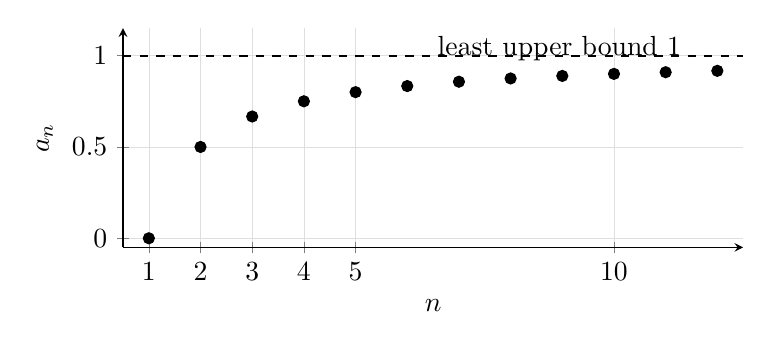
\begin{tikzpicture}
\begin{axis}[
    width=0.78\textwidth,
    height=0.36\textwidth,
    xmin=0.5, xmax=12.5,
    ymin=-0.05, ymax=1.15,
    axis lines=left,
    xlabel={\(n\)},
    ylabel={\(a_n\)},
    xtick={1,2,3,4,5,10},
    ytick={0,0.5,1},
    grid=both,
    grid style={line width=.1pt, draw=gray!25},
]
\addplot[only marks, mark=*] coordinates {
    (1,0)
    (2,0.5)
    (3,0.6667)
    (4,0.75)
    (5,0.8)
    (6,0.8333)
    (7,0.8571)
    (8,0.875)
    (9,0.8889)
    (10,0.9)
    (11,0.9091)
    (12,0.9167)
};
\addplot[thick, dashed, domain=0.5:12.5, samples=2] {1};
\node[anchor=west] at (axis cs:6.4,1.04) {least upper bound \(1\)};
\end{axis}
\end{tikzpicture}
\caption{An increasing sequence trapped below an upper bound must approach its least upper bound.}
\label{fig:monotone-sequence-approaches-sup}
\end{figure}

\subsection{The theorem}
\label{appsubsec:monotone-convergence-theorem-statement}

\begin{quote}
\textbf{Monotone Convergence Theorem.}

If an increasing sequence is bounded above, then it converges.

If a decreasing sequence is bounded below, then it converges.
\end{quote}

The theorem is not saying that every sequence converges.  It is saying that two
conditions together force convergence:

\[
\boxed{
\text{one direction of motion}+\text{a barrier}
\quad\Longrightarrow\quad
\text{a limit.}
}
\]

\paragraph{Proof for increasing sequences.}
Let

\[
a_1\le a_2\le a_3\le\cdots
\]

be an increasing sequence that is bounded above.

Consider the set of its terms:

\[
A=\{a_n:n=1,2,3,\ldots\}.
\]

This set is nonempty and bounded above.  By the Least Upper Bound Property, it has a
least upper bound.  Call it \(L\):

\[
L=\sup A.
\]

We will prove that

\[
a_n\to L.
\]

Let \(\varepsilon>0\).  By the approximation property of the supremum, there is some
term \(a_N\) such that

\[
L-\varepsilon<a_N\le L.
\]

Since the sequence is increasing, every later term satisfies

\[
a_n\ge a_N
\qquad\text{for }n\ge N.
\]

Also, since \(L\) is an upper bound, every term satisfies

\[
a_n\le L.
\]

Therefore, for every \(n\ge N\),

\[
L-\varepsilon<a_n\le L.
\]

This gives

\[
|a_n-L|<\varepsilon.
\]

So

\[
a_n\to L.
\]

\paragraph{Proof for decreasing sequences.}
If

\[
b_1\ge b_2\ge b_3\ge\cdots
\]

and the sequence is bounded below, then the set of terms has an infimum.  Call it
\(M\):

\[
M=\inf\{b_n:n=1,2,3,\ldots\}.
\]

The same argument from below shows that

\[
b_n\to M.
\]

\subsection{Why the hypotheses matter}
\label{appsubsec:monotone-theorem-hypotheses}

Both hypotheses are needed.

\paragraph{Increasing but not bounded.}
The sequence

\[
a_n=n
\]

is increasing, but it is not bounded above.  It does not converge to a real number.

\[
1,\ 2,\ 3,\ 4,\ldots
\]

It escapes.

\paragraph{Bounded but not monotone.}
The sequence

\[
b_n=(-1)^n
\]

is bounded:

\[
-1\le b_n\le 1.
\]

But it is not monotone.  It keeps jumping:

\[
-1,\ 1,\ -1,\ 1,\ldots.
\]

It does not converge.

\begin{quote}
\textbf{The theorem needs both parts.}
A barrier without one-direction motion is not enough.  One-direction motion without a
barrier is not enough.
\end{quote}

\subsection{Nested intervals}
\label{appsubsec:nested-intervals}

The Monotone Convergence Theorem gives a useful interval principle.

Suppose we have closed intervals

\[
I_n=[L_n,R_n]
\]

such that each interval sits inside the previous one:

\[
I_1\supset I_2\supset I_3\supset\cdots.
\]

Then the left endpoints move right or stay fixed:

\[
L_1\le L_2\le L_3\le\cdots,
\]

and the right endpoints move left or stay fixed:

\[
R_1\ge R_2\ge R_3\ge\cdots.
\]

If the interval lengths shrink to \(0\),

\[
R_n-L_n\to0,
\]

then the intervals trap exactly one real number.

\begin{quote}
\textbf{Nested Interval Principle, shrinking version.}
If

\[
[L_1,R_1]\supset [L_2,R_2]\supset [L_3,R_3]\supset\cdots
\]

and

\[
R_n-L_n\to0,
\]

then there is exactly one real number \(c\) that lies in every interval.
\end{quote}

\paragraph{Proof sketch.}
The sequence \(L_n\) is increasing and bounded above by \(R_1\), so it converges.
The sequence \(R_n\) is decreasing and bounded below by \(L_1\), so it converges.

Let

\[
L_n\to c
\qquad\text{and}\qquad
R_n\to d.
\]

Since

\[
R_n-L_n\to0,
\]

we must have

\[
d-c=0,
\]

so

\[
c=d.
\]

Thus the left and right endpoints squeeze down to one number.

\begin{figure}[h]
\centering
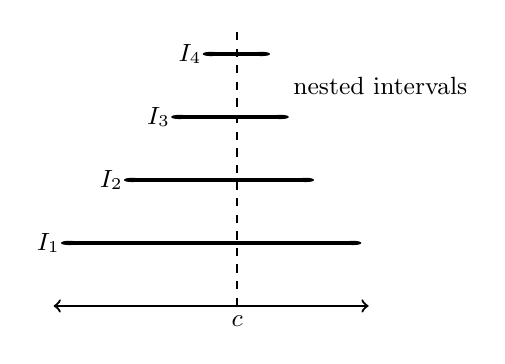
\begin{tikzpicture}[xscale=4.0, yscale=0.8, every node/.style={font=\small}]
  \draw[<->, thick] (0.75,0) -- (1.75,0);
  \foreach \y/\l/\r/\name in {1/0.8/1.7/{\(I_1\)},2/1.0/1.55/{\(I_2\)},3/1.15/1.47/{\(I_3\)},4/1.25/1.41/{\(I_4\)}} {
    \draw[very thick] (\l,\y) -- (\r,\y);
    \draw[fill=black] (\l,\y) circle (0.7pt);
    \draw[fill=black] (\r,\y) circle (0.7pt);
    \node[left] at (\l,\y) {\name};
  }
  \draw[dashed, thick] (1.333,0) -- (1.333,4.4);
  \node[below] at (1.333,0) {\(c\)};
  \node[right] at (1.48,3.5) {nested intervals};
\end{tikzpicture}
\caption{Shrinking nested closed intervals trap a single real number.}
\label{fig:nested-intervals-shrink}
\end{figure}

This is the proof engine behind bisection.

\section{Bolzano's Theorem and Bisection}
\label{appsec:bolzano-bisection}

The Intermediate Value Theorem says that a continuous graph cannot jump over a
height.  A special and extremely useful case is the root case.

If a continuous function changes sign, then it must be zero somewhere in between.

\subsection{Bolzano's theorem}
\label{appsubsec:bolzano-theorem}

\begin{quote}
\textbf{Bolzano's Theorem.}
Suppose \(f\) is continuous on \([a,b]\).  If

\[
f(a)<0
\qquad\text{and}\qquad
f(b)>0,
\]

then there is at least one number \(c\in(a,b)\) such that

\[
f(c)=0.
\]

The same conclusion holds if the signs are reversed.
\end{quote}

This is the Intermediate Value Theorem with the intermediate value \(0\).

\begin{figure}[h]
\centering
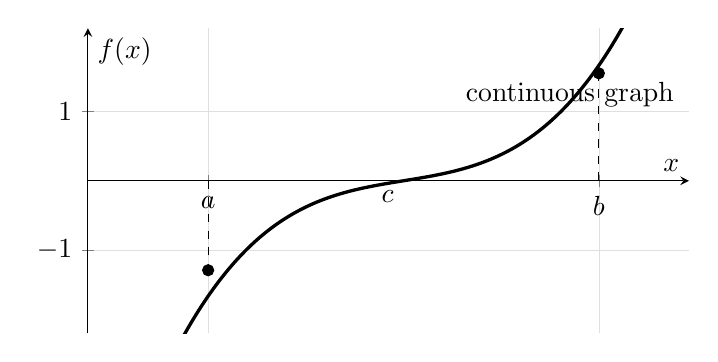
\begin{tikzpicture}
\begin{axis}[
    width=0.76\textwidth,
    height=0.45\textwidth,
    xmin=0, xmax=4,
    ymin=-2.2, ymax=2.2,
    axis lines=middle,
    xlabel={\(x\)},
    ylabel={\(f(x)\)},
    xtick={0.8,3.4},
    xticklabels={\(a\),\(b\)},
    ytick={-1,0,1},
    grid=both,
    grid style={line width=.1pt, draw=gray!25},
]
\addplot[very thick, domain=0.55:3.6, samples=150] {0.55*(x-2.1)^3 + 0.35*(x-2.1)};
\addplot[only marks, mark=*] coordinates {(0.8,-1.29) (3.4,1.55)};
\draw[dashed] (axis cs:0.8,0) -- (axis cs:0.8,-1.29);
\draw[dashed] (axis cs:3.4,0) -- (axis cs:3.4,1.55);
\node[anchor=north east] at (axis cs:2.1,0) {\(c\)};
\node[anchor=west] at (axis cs:2.45,1.25) {continuous graph};
\end{axis}
\end{tikzpicture}
\caption{A continuous graph that goes from negative to positive must cross the \(x\)-axis.}
\label{fig:bolzano-crossing}
\end{figure}

\subsection{Proof by bisection}
\label{appsubsec:bolzano-proof-bisection}

Assume

\[
f(a)<0
\qquad\text{and}\qquad
f(b)>0.
\]

Set

\[
L_1=a,
\qquad
R_1=b.
\]

The interval

\[
[L_1,R_1]
\]

has a sign change.

Now bisect the interval.  Let

\[
M_1=\frac{L_1+R_1}{2}.
\]

There are three possibilities.

If

\[
f(M_1)=0,
\]

then we have found a root.

If

\[
f(M_1)>0,
\]

then the sign change occurs on

\[
[L_1,M_1],
\]

so we choose

\[
L_2=L_1,
\qquad
R_2=M_1.
\]

If

\[
f(M_1)<0,
\]

then the sign change occurs on

\[
[M_1,R_1],
\]

so we choose

\[
L_2=M_1,
\qquad
R_2=R_1.
\]

Repeat this process.

Unless we find a root exactly at a midpoint, we create nested intervals

\[
[L_1,R_1]\supset [L_2,R_2]\supset [L_3,R_3]\supset\cdots
\]

such that

\[
f(L_n)\le0
\qquad\text{and}\qquad
f(R_n)\ge0
\]

for every \(n\).

Each bisection cuts the length in half:

\[
R_n-L_n=\frac{b-a}{2^{n-1}}.
\]

So

\[
R_n-L_n\to0.
\]

By the Nested Interval Principle, the intervals trap one number \(c\).  Thus

\[
L_n\to c
\qquad\text{and}\qquad
R_n\to c.
\]

Since \(f\) is continuous,

\[
f(L_n)\to f(c)
\qquad\text{and}\qquad
f(R_n)\to f(c).
\]

But

\[
f(L_n)\le0
\]

for every \(n\), so the limit satisfies

\[
f(c)\le0.
\]

Also,

\[
f(R_n)\ge0
\]

for every \(n\), so the limit satisfies

\[
f(c)\ge0.
\]

Therefore

\[
f(c)=0.
\]

That proves Bolzano's Theorem.

\begin{quote}
\textbf{The proof is also an algorithm.}
The same bisection process that proves the root exists also gives numerical
approximations to the root.
\end{quote}

\subsection{Bisection error}
\label{appsubsec:bisection-error}

After \(N\) completed bisections, the interval containing the root has length

\[
\boxed{
\frac{b-a}{2^N}.
}
\]

If we report the midpoint of the final interval as our approximation, then the true root
is at most half an interval length away.  Therefore the midpoint error is at most

\[
\boxed{
\frac{b-a}{2^{N+1}}.
}
\]

\paragraph{Example.}
Use bisection to locate a root of

\[
p(x)=x^3-x-1
\]

in the interval \([1,2]\).

First check the signs:

\[
p(1)=1-1-1=-1<0,
\]

and

\[
p(2)=8-2-1=5>0.
\]

So there is a root in \((1,2)\).

\begin{center}
\renewcommand{\arraystretch}{1.45}
\begin{tabular}{c|c|c|c|c|c}
\textbf{step} & \(L\) & \(R\) & \(M=\dfrac{L+R}{2}\) & \(p(M)\) & \textbf{next interval} \\ \hline
\(0\) & \(1\) & \(2\) & \(1.5\) & \(0.875\) & \([1,1.5]\) \\
\(1\) & \(1\) & \(1.5\) & \(1.25\) & \(-0.296875\) & \([1.25,1.5]\) \\
\(2\) & \(1.25\) & \(1.5\) & \(1.375\) & \(0.224609375\) & \([1.25,1.375]\) \\
\(3\) & \(1.25\) & \(1.375\) & \(1.3125\) & \(-0.051513672\) & \([1.3125,1.375]\)
\end{tabular}
\end{center}

After four completed bisections, the root lies in

\[
[1.3125,1.375].
\]

The interval length is

\[
\frac1{2^4}=\frac1{16}=0.0625.
\]

If we use the midpoint

\[
\frac{1.3125+1.375}{2}=1.34375,
\]

then the error is at most

\[
\frac{0.0625}{2}=0.03125.
\]

More bisections improve the guarantee.

\subsection{Why continuity matters}
\label{appsubsec:bolzano-continuity-matters}

Bolzano's Theorem fails without continuity.

Define

\[
J(x)=
\begin{cases}
-1, & x<0,\\
1, & x\ge0.
\end{cases}
\]

Then

\[
J(-1)=-1<0
\qquad\text{and}\qquad
J(1)=1>0.
\]

But there is no \(c\in[-1,1]\) with

\[
J(c)=0.
\]

The function jumps over \(0\).

\begin{figure}[h]
\centering
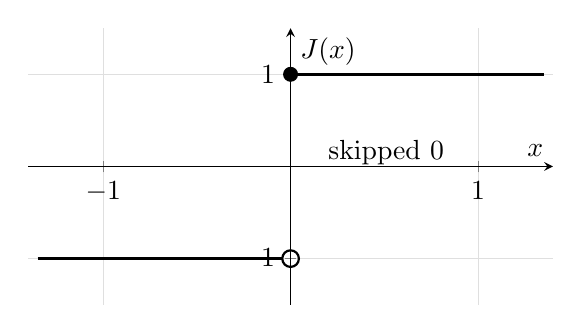
\begin{tikzpicture}
\begin{axis}[
    width=0.68\textwidth,
    height=0.42\textwidth,
    xmin=-1.4, xmax=1.4,
    ymin=-1.5, ymax=1.5,
    axis lines=middle,
    xlabel={\(x\)},
    ylabel={\(J(x)\)},
    xtick={-1,0,1},
    ytick={-1,0,1},
    grid=both,
    grid style={line width=.1pt, draw=gray!25},
]
\addplot[very thick, domain=-1.35:-0.04, samples=2] {-1};
\addplot[very thick, domain=0:1.35, samples=2] {1};
\addplot[only marks, mark=o, mark size=3pt, thick] coordinates {(0,-1)};
\addplot[only marks, mark=*, mark size=2.5pt] coordinates {(0,1)};
\draw[dashed] (axis cs:-1.35,0) -- (axis cs:1.35,0);
\node[anchor=west] at (axis cs:0.15,0.15) {skipped \(0\)};
\end{axis}
\end{tikzpicture}
\caption{A jump discontinuity can change sign without crossing \(0\).}
\label{fig:bolzano-fails-jump}
\end{figure}

The theorem is a no-jump theorem.

\section{The Extreme Value Theorem: Proof Outline}
\label{appsec:evt-proof-outline}

The Extreme Value Theorem says that a continuous function on a closed and bounded
interval reaches its highest and lowest values.

The theorem sounds visually obvious.  But each word is doing work.

\[
\boxed{
\text{continuous on a closed bounded interval}
\quad\Longrightarrow\quad
\text{absolute max and min are attained.}
}
\]

This section explains why completeness is hiding behind that statement.

\subsection{Statement of the theorem}
\label{appsubsec:evt-statement}

\begin{quote}
\textbf{Extreme Value Theorem.}
If \(f\) is continuous on the closed interval \([a,b]\), then \(f\) has an absolute maximum
and an absolute minimum on \([a,b]\).

That is, there are points \(c,d\in[a,b]\) such that

\[
f(c)\le f(x)\le f(d)
\]

for every \(x\in[a,b]\).
\end{quote}

The theorem has two parts:

\[
\text{the values are bounded}
\]

and

\[
\text{the top and bottom values are actually reached.}
\]

\subsection{Why the function is bounded}
\label{appsubsec:evt-bounded-proof}

First we explain why a continuous function on \([a,b]\) cannot blow up.

Suppose, for contradiction, that \(f\) is not bounded above on \([a,b]\).

Bisect the interval \([a,b]\).  If \(f\) were bounded above on both halves, then it would
be bounded above on the whole interval.  So at least one half must still have no upper
bound.

Choose such a half.  Bisect it again.  Again choose a half where \(f\) is not bounded
above.

This produces nested intervals

\[
I_1\supset I_2\supset I_3\supset\cdots
\]

whose lengths shrink to \(0\).  By the Nested Interval Principle, they trap a point
\(c\in[a,b]\).

Because \(f\) is continuous at \(c\), there is a small interval around \(c\) on which the
values of \(f\) stay close to \(f(c)\).  For example, there is a \(\delta>0\) such that

\[
|x-c|<\delta
\quad\Longrightarrow\quad
|f(x)-f(c)|<1.
\]

So on that small interval,

\[
f(c)-1<f(x)<f(c)+1.
\]

Thus \(f\) is bounded there.

But the nested intervals eventually become so short that one of them lies entirely inside

\[
(c-\delta,c+\delta).
\]

That chosen interval was supposed to be one where \(f\) is not bounded above.  This is
a contradiction.

Therefore \(f\) must be bounded above.

The same argument applied to \(-f\) shows that \(f\) is bounded below.

\subsection{Why the maximum is reached}
\label{appsubsec:evt-maximum-proof}

Since \(f\) is bounded above on \([a,b]\), the set of values

\[
V=\{f(x):x\in[a,b]\}
\]

is nonempty and bounded above.  By the Least Upper Bound Property, it has a
supremum.  Call it \(M\):

\[
M=\sup V.
\]

So \(M\) is the least upper bound of all function values.

We must show that some point \(c\in[a,b]\) actually satisfies

\[
f(c)=M.
\]

If the graph only approached \(M\) but never reached it, then \(M\) would be a
supremum but not a maximum.  The closed interval and continuity prevent that.

Here is the bisection idea.

Start with

\[
I_1=[a,b].
\]

The supremum of \(f\) on \(I_1\) is \(M\).  Bisect \(I_1\).  At least one half must still
have supremum \(M\).  If both halves had supremum less than \(M\), then their union
would also have supremum less than \(M\), which is impossible.

Choose a half whose supremum is still \(M\).  Call it \(I_2\).  Repeat.

This creates nested intervals

\[
I_1\supset I_2\supset I_3\supset\cdots
\]

with lengths tending to \(0\), and with the property that the supremum of \(f\) on each
\(I_n\) is \(M\).

By the Nested Interval Principle, these intervals trap a point \(c\).

Now suppose

\[
f(c)<M.
\]

Choose

\[
\varepsilon=\frac{M-f(c)}{2}>0.
\]

By continuity at \(c\), there is a \(\delta>0\) such that

\[
|x-c|<\delta
\quad\Longrightarrow\quad
|f(x)-f(c)|<\varepsilon.
\]

Then every such \(x\) satisfies

\[
f(x)<f(c)+\varepsilon
=
\frac{f(c)+M}{2}
<
M.
\]

For large \(n\), the interval \(I_n\) lies inside \((c-\delta,c+\delta)\).  On that whole
interval, \(f(x)\) is bounded above by a number smaller than \(M\).

That contradicts the way \(I_n\) was chosen: its supremum was supposed to be \(M\).

Therefore the assumption \(f(c)<M\) is impossible.  Hence

\[
f(c)=M.
\]

So \(f\) reaches its absolute maximum.

The absolute minimum follows by applying the maximum argument to

\[
-f.
\]

\begin{figure}[h]
\centering
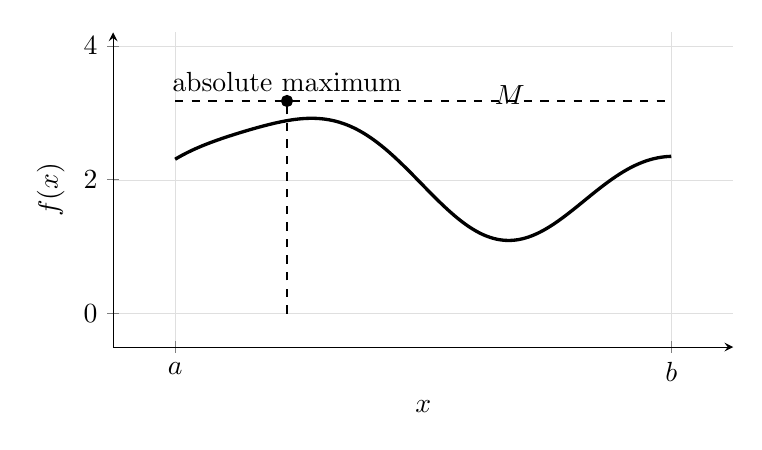
\begin{tikzpicture}
\begin{axis}[
    width=0.78\textwidth,
    height=0.46\textwidth,
    xmin=0, xmax=5,
    ymin=-0.5, ymax=4.2,
    axis lines=left,
    xlabel={\(x\)},
    ylabel={\(f(x)\)},
    xtick={0.5,4.5},
    xticklabels={\(a\),\(b\)},
    ytick={0,2,4},
    grid=both,
    grid style={line width=.1pt, draw=gray!25},
]
\addplot[very thick, domain=0.5:4.5, samples=220] {2.4 + 1.0*sin(deg(1.5*x)) - 0.18*(x-2.6)^2 + 0.25*cos(deg(3*x))};
\addplot[only marks, mark=*] coordinates {(1.402,3.176)};
\draw[dashed] (axis cs:1.402,0) -- (axis cs:1.402,3.176);
\draw[dashed] (axis cs:0.5,3.176) -- (axis cs:4.5,3.176);
\node[anchor=south] at (axis cs:1.402,3.176) {absolute maximum};
\node[anchor=west] at (axis cs:3.0,3.26) {\(M\)};
\end{axis}
\end{tikzpicture}
\caption{Continuity on a closed interval forces the supremum of the values to be reached.}
\label{fig:evt-maximum-reached}
\end{figure}

\subsection{Why the hypotheses matter}
\label{appsubsec:evt-hypotheses-matter}

The hypotheses of the Extreme Value Theorem cannot be removed.

\paragraph{Missing endpoint.}
The function

\[
f(x)=x
\]

on

\[
(0,1)
\]

is continuous on its domain, but it has no absolute maximum and no absolute minimum.

The values approach \(1\), but never reach \(1\).  They approach \(0\), but never reach
\(0\).

The problem is that the interval is not closed.

\paragraph{Unbounded interval.}
The function

\[
f(x)=x
\]

on

\[
[0,\infty)
\]

is continuous and the interval is closed, but the interval is not bounded.  The function
has a minimum value \(0\), but no maximum.

\paragraph{Discontinuity.}
Define

\[
g(x)=
\begin{cases}
x, & 0\le x<1,\\
0, & x=1.
\end{cases}
\]

The function is defined on the closed bounded interval \([0,1]\), but it is not
continuous at \(1\).  Its values get arbitrarily close to \(1\), but no input gives value
\(1\).

So \(g\) has no absolute maximum.

\begin{quote}
\textbf{Closed, bounded, continuous.}
Each word in the Extreme Value Theorem protects against a different failure.
\end{quote}

\section{Uniform Continuity on Closed Intervals}
\label{appsec:uniform-continuity}

Continuity at a point says:

\[
\text{near this input, nearby inputs give nearby outputs.}
\]

Uniform continuity says something stronger:

\[
\text{one input tolerance works everywhere on the interval.}
\]

This distinction matters when we want to control error across a whole interval, as in
Riemann sums, numerical integration, and approximation.

\subsection{Pointwise continuity versus uniform continuity}
\label{appsubsec:pointwise-vs-uniform-continuity}

A function \(f\) is continuous at \(c\) if, for every \(\varepsilon>0\), there is a
\(\delta>0\) such that

\[
|x-c|<\delta
\quad\Longrightarrow\quad
|f(x)-f(c)|<\varepsilon.
\]

The number \(\delta\) may depend on the point \(c\).

Uniform continuity asks for one \(\delta\) that works for all points in the set.

\begin{quote}
\textbf{Uniform continuity.}
A function \(f\) is \emph{uniformly continuous} on a set \(S\) if, for every
\(\varepsilon>0\), there is a \(\delta>0\) such that whenever \(x,y\in S\),

\[
|x-y|<\delta
\]

we have

\[
|f(x)-f(y)|<\varepsilon.
\]
\end{quote}

The order of the quantifiers is the whole point.

For ordinary continuity, the point is chosen first, and \(\delta\) may depend on that
point.

For uniform continuity, \(\varepsilon\) is chosen first, and then one \(\delta\) must work
for every pair of points in the set.

\begin{center}
\renewcommand{\arraystretch}{1.7}
\begin{tabular}{p{0.42\textwidth}|p{0.42\textwidth}}
\textbf{continuity at each point} & \textbf{uniform continuity} \\ \hline
\(\delta\) may change from point to point & one \(\delta\) works everywhere \\ \hline
local control & global control on the set \\ \hline
enough for tangent behavior at a point & needed for reliable interval-wide error control
\end{tabular}
\end{center}

\subsection{A simple uniform continuity estimate}
\label{appsubsec:simple-uniform-estimate}

Let

\[
f(x)=x^2
\]

on the interval

\[
[0,10].
\]

For \(x,y\in[0,10]\),

\[
|x^2-y^2|
=
|x-y||x+y|.
\]

Since \(0\le x\le10\) and \(0\le y\le10\),

\[
|x+y|\le20.
\]

So

\[
|x^2-y^2|\le20|x-y|.
\]

Given \(\varepsilon>0\), choose

\[
\delta=\frac{\varepsilon}{20}.
\]

Then

\[
|x-y|<\delta
\]

implies

\[
|x^2-y^2|<20\cdot\frac{\varepsilon}{20}=\varepsilon.
\]

Thus \(x^2\) is uniformly continuous on \([0,10]\).

The bounded interval mattered.  It gave the uniform estimate

\[
|x+y|\le20.
\]

\subsection{A continuous function that is not uniformly continuous}
\label{appsubsec:not-uniform-continuity-examples}

The function

\[
f(x)=\frac1x
\]

is continuous on the open interval

\[
(0,1).
\]

But it is not uniformly continuous there.

To see the problem, compare the two nearby numbers

\[
x_n=\frac1n
\qquad\text{and}\qquad
y_n=\frac1{n+1}.
\]

Their distance is

\[
|x_n-y_n|
=
\left|\frac1n-\frac1{n+1}\right|
=
\frac1{n(n+1)}.
\]

This tends to \(0\).

But the function values differ by

\[
\left|f(x_n)-f(y_n)\right|
=
|n-(n+1)|
=
1.
\]

So the inputs can be made arbitrarily close while the outputs stay \(1\) unit apart.

Therefore no single \(\delta\) can guarantee output error less than, say,

\[
\varepsilon=\frac12.
\]

\[
\boxed{
\frac1x\text{ is continuous on }(0,1)\text{ but not uniformly continuous there.}
}
\]

The issue is the missing endpoint \(0\).  Near \(0\), the graph becomes steeper and
steeper.

\begin{figure}[h]
\centering
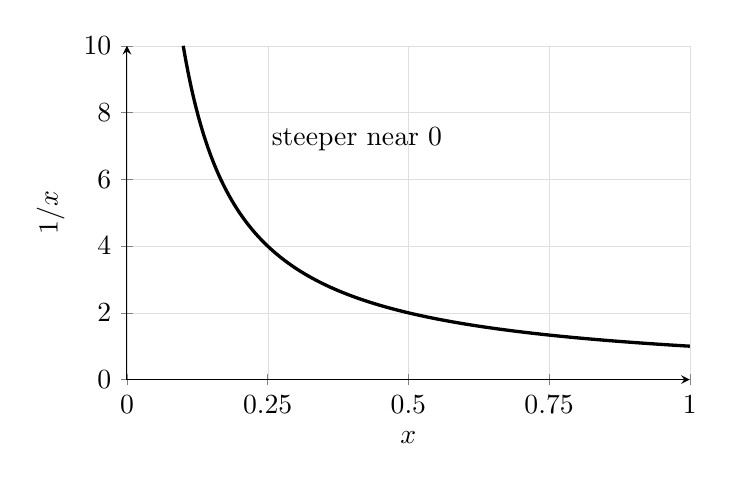
\begin{tikzpicture}
\begin{axis}[
    width=0.72\textwidth,
    height=0.48\textwidth,
    xmin=0, xmax=1,
    ymin=0, ymax=10,
    axis lines=left,
    xlabel={\(x\)},
    ylabel={\(1/x\)},
    xtick={0,0.25,0.5,0.75,1},
    ytick={0,2,4,6,8,10},
    grid=both,
    grid style={line width=.1pt, draw=gray!25},
]
\addplot[very thick, domain=0.1:1, samples=200] {1/x};
\node[anchor=west] at (axis cs:0.24,7.2) {steeper near \(0\)};
\end{axis}
\end{tikzpicture}
\caption{The function \(1/x\) is continuous on \((0,1)\), but no single input tolerance works everywhere.}
\label{fig:one-over-x-not-uniform}
\end{figure}

\subsection{The theorem on closed intervals}
\label{appsubsec:uniform-continuity-theorem}

Closed bounded intervals prevent the kind of escape seen in \(1/x\) on \((0,1)\).

\begin{quote}
\textbf{Uniform Continuity Theorem.}
If \(f\) is continuous on a closed interval \([a,b]\), then \(f\) is uniformly continuous
on \([a,b]\).
\end{quote}

This theorem says that point-by-point continuity becomes interval-wide control when
the domain is closed and bounded.

\subsection{Finite covering lemma}
\label{appsubsec:finite-covering-lemma}

The proof uses one compactness fact about closed intervals.

\begin{quote}
\textbf{Finite covering lemma for closed intervals.}
Suppose every point of \([a,b]\) lies in at least one open interval from some collection
of open intervals.  Then finitely many of those open intervals already cover all of
\([a,b]\).
\end{quote}

\paragraph{Proof idea.}
If no finite subcollection covered \([a,b]\), bisect \([a,b]\).  At least one half would
also fail to be covered by finitely many intervals.  Choose such a half and repeat.

This creates nested closed intervals whose lengths shrink to \(0\).  They trap a point
\(c\in[a,b]\).

But \(c\) lies in one of the open intervals from the original cover.  Since that interval is
open, it contains a small neighborhood around \(c\).  Eventually the nested interval is
so short that it lies entirely inside that one open interval.  Then that nested interval is
covered by a single member of the cover, contradicting how it was chosen.

So a finite subcover must exist.

This is another place where the completeness of the real line is doing hidden work.

\subsection{Proof of uniform continuity}
\label{appsubsec:uniform-continuity-proof}

Let \(f\) be continuous on \([a,b]\).  We prove that \(f\) is uniformly continuous.

Choose an arbitrary

\[
\varepsilon>0.
\]

For each point \(c\in[a,b]\), continuity at \(c\) gives a number \(\rho_c>0\) such that

\[
|x-c|<\rho_c
\quad\Longrightarrow\quad
|f(x)-f(c)|<\frac{\varepsilon}{2}.
\]

Now form the smaller open interval

\[
U_c=\left(c-\frac{\rho_c}{2},c+\frac{\rho_c}{2}\right).
\]

As \(c\) runs through \([a,b]\), these intervals cover \([a,b]\).

By the finite covering lemma, finitely many of them cover the whole interval:

\[
U_{c_1},U_{c_2},\ldots,U_{c_N}.
\]

Now define

\[
\delta=\frac12\min\{\rho_{c_1},\rho_{c_2},\ldots,\rho_{c_N}\}.
\]

This \(\delta\) is positive because it is half the minimum of finitely many positive
numbers.

Suppose \(x,y\in[a,b]\) and

\[
|x-y|<\delta.
\]

Since the finitely many \(U_{c_j}\) cover \([a,b]\), the point \(x\) lies in one of them.
Say

\[
x\in U_{c_j}.
\]

Then

\[
|x-c_j|<\frac{\rho_{c_j}}{2}.
\]

Also,

\[
|y-c_j|
\le
|y-x|+|x-c_j|
<
\delta+\frac{\rho_{c_j}}{2}
\le
\frac{\rho_{c_j}}{2}+\frac{\rho_{c_j}}{2}
=
\rho_{c_j}.
\]

Thus both \(x\) and \(y\) are within \(\rho_{c_j}\) of \(c_j\).  Therefore

\[
|f(x)-f(c_j)|<\frac{\varepsilon}{2}
\]

and

\[
|f(y)-f(c_j)|<\frac{\varepsilon}{2}.
\]

By the triangle inequality,

\[
|f(x)-f(y)|
\le
|f(x)-f(c_j)|+|f(c_j)-f(y)|
<
\frac{\varepsilon}{2}+\frac{\varepsilon}{2}
=
\varepsilon.
\]

So one \(\delta\) works for all \(x,y\in[a,b]\).  Hence \(f\) is uniformly continuous.

\begin{quote}
\textbf{Why this matters.}
Uniform continuity is the reason that, on a closed interval, making subintervals short
enough controls the function's oscillation everywhere.  That is one of the quiet
foundations behind Riemann sums and numerical integration.
\end{quote}

\section{Practice problems}
\label{appsec:proofs-completeness-practice}

\subsection*{Least upper bounds}

\begin{enumerate}
\item For each set, find the supremum and infimum.  State whether each is actually
attained as a maximum or minimum.

\[
A=(2,5),
\]

\[
B=[2,5),
\]

\[
C=\left\{1-\frac1n:n=1,2,3,\ldots\right\},
\]

\[
D=\{x\in\mathbb R:x\ge0\text{ and }x^2<7\}.
\]

\item Let \(s=\sup A\).  Prove that for every \(\varepsilon>0\), there is an \(a\in A\)
such that

\[
s-\varepsilon<a.
\]

\item Let \(A\) be nonempty and bounded below.  Explain why

\[
\inf A=-\sup(-A).
\]
\end{enumerate}

\subsection*{Monotone convergence}

\begin{enumerate}
\item Prove that

\[
a_n=1-\frac1n
\]

is increasing and bounded above.  Then use the Monotone Convergence Theorem to find
its limit.

\item Give an example of an increasing sequence that does not converge.

\item Give an example of a bounded sequence that does not converge.

\item Suppose

\[
[L_1,R_1]\supset[L_2,R_2]\supset[L_3,R_3]\supset\cdots
\]

and

\[
R_n-L_n\to0.
\]

Explain why the intervals contain exactly one common point.
\end{enumerate}

\subsection*{Bolzano's theorem and bisection}

\begin{enumerate}
\item Use Bolzano's Theorem to prove that

\[
x^5+x-1=0
\]

has at least one solution in \((0,1)\).

\item Prove that the solution in the previous problem is unique.

\item Bisection starts with an interval of length \(1\).  After \(N\) bisections, what is
the interval length?

\item If the midpoint is reported after \(N\) bisections starting from an interval of
length \(1\), what is the maximum possible error?

\item How many bisections are enough to guarantee midpoint error less than

\[
10^{-5}
\]

when the starting interval has length \(1\)?

\item Give an example of a function with

\[
f(0)<0
\qquad\text{and}\qquad
f(1)>0,
\]

but with no zero in \((0,1)\).  Which hypothesis of Bolzano's Theorem fails?
\end{enumerate}

\subsection*{Extreme Value Theorem}

\begin{enumerate}
\item Explain why

\[
f(x)=x
\]

has no absolute maximum on \((0,1)\).  Which hypothesis of the Extreme Value Theorem
is missing?

\item Explain why

\[
f(x)=x
\]

has no absolute maximum on \([0,\infty)\).  Which hypothesis is missing?

\item Define

\[
g(x)=
\begin{cases}
x, & 0\le x<1,\\
0, & x=1.
\end{cases}
\]

Explain why \(g\) has no absolute maximum on \([0,1]\).  Which hypothesis is missing?

\item Let \(f\) be continuous on \([a,b]\), and let

\[
M=\sup\{f(x):x\in[a,b]\}.
\]

In the nested-interval proof of the Extreme Value Theorem, explain why the assumption

\[
f(c)<M
\]

contradicts continuity at \(c\).
\end{enumerate}

\subsection*{Uniform continuity}

\begin{enumerate}
\item Prove directly that

\[
f(x)=x^2
\]

is uniformly continuous on \([0,4]\).

\item Show that

\[
f(x)=x^2
\]

is not uniformly continuous on \(\mathbb R\).  Use the pairs

\[
x_n=n,
\qquad
y_n=n+\frac1n.
\]

\item Show that

\[
f(x)=\frac1x
\]

is not uniformly continuous on \((0,1)\).  Use the pairs

\[
x_n=\frac1n,
\qquad
y_n=\frac1{n+1}.
\]

\item Explain in words why every continuous function on \([a,b]\) is uniformly
continuous, but a continuous function on \((a,b)\) need not be.
\end{enumerate}

\section*{Answers to Appendix D practice problems}
\label{ans:appendix-d-practice}

\subsection*{Least upper bounds}

\begin{enumerate}
\item
For

\[
A=(2,5),
\]

we have

\[
\inf A=2,
\qquad
\sup A=5.
\]

Neither is attained.

For

\[
B=[2,5),
\]

we have

\[
\inf B=2,
\qquad
\sup B=5.
\]

The infimum is attained as a minimum.  The supremum is not attained.

For

\[
C=\left\{1-\frac1n:n=1,2,3,\ldots\right\},
\]

the terms are

\[
0,\ \frac12,\ \frac23,\ \frac34,\ldots.
\]

Thus

\[
\inf C=0,
\qquad
\sup C=1.
\]

The infimum is attained at \(n=1\).  The supremum is not attained.

For

\[
D=\{x\in\mathbb R:x\ge0\text{ and }x^2<7\},
\]

we have

\[
\inf D=0,
\qquad
\sup D=\sqrt7.
\]

The infimum is attained.  The supremum is not attained because \(x^2<7\), not
\(x^2\le7\).

\item
If no element of \(A\) satisfied

\[
s-\varepsilon<a,
\]

then every \(a\in A\) would satisfy

\[
a\le s-\varepsilon.
\]

That would make \(s-\varepsilon\) an upper bound for \(A\), smaller than \(s\).  This
contradicts

\[
s=\sup A.
\]

Therefore some \(a\in A\) satisfies

\[
s-\varepsilon<a.
\]

\item
Let

\[
-A=\{-a:a\in A\}.
\]

Lower bounds for \(A\) become upper bounds for \(-A\) after multiplying by \(-1\).
So the greatest lower bound of \(A\) is the negative of the least upper bound of
\(-A\):

\[
\inf A=-\sup(-A).
\]
\end{enumerate}

\subsection*{Monotone convergence}

\begin{enumerate}
\item
For

\[
a_n=1-\frac1n,
\]

we compute

\[
a_{n+1}-a_n
=
\left(1-\frac1{n+1}\right)-\left(1-\frac1n\right)
=
\frac1n-\frac1{n+1}
=
\frac1{n(n+1)}>0.
\]

So the sequence is increasing.

Also,

\[
a_n=1-\frac1n<1,
\]

so it is bounded above by \(1\).  By the Monotone Convergence Theorem, it converges.
Its least upper bound is \(1\), so

\[
\boxed{
\lim_{n\to\infty}\left(1-\frac1n\right)=1.
}
\]

\item
The sequence

\[
a_n=n
\]

is increasing but does not converge, because it is not bounded above.

\item
The sequence

\[
a_n=(-1)^n
\]

is bounded but does not converge, because it oscillates between \(-1\) and \(1\).

\item
The left endpoints \(L_n\) form an increasing bounded sequence, and the right endpoints
\(R_n\) form a decreasing bounded sequence.  Therefore both converge.  Since

\[
R_n-L_n\to0,
\]

their limits are equal.  That common limit is the only point contained in all the
intervals.
\end{enumerate}

\subsection*{Bolzano's theorem and bisection}

\begin{enumerate}
\item
Let

\[
f(x)=x^5+x-1.
\]

Then

\[
f(0)=-1<0
\]

and

\[
f(1)=1+1-1=1>0.
\]

Since \(f\) is continuous on \([0,1]\), Bolzano's Theorem guarantees a number
\(c\in(0,1)\) such that

\[
f(c)=0.
\]

\item
The derivative is

\[
f'(x)=5x^4+1.
\]

Since

\[
5x^4+1>0
\]

for every real \(x\), the function is strictly increasing.  A strictly increasing function
can cross \(0\) at most once.  Therefore the solution in \((0,1)\) is unique.

\item
After \(N\) bisections, the interval length is

\[
\boxed{
\frac1{2^N}.
}
\]

\item
The midpoint error is at most half the interval length:

\[
\boxed{
\frac1{2^{N+1}}.
}
\]

\item
We need

\[
\frac1{2^{N+1}}<10^{-5}.
\]

Equivalently,

\[
2^{N+1}>100000.
\]

Since

\[
2^{16}=65536
\qquad\text{and}\qquad
2^{17}=131072,
\]

we need

\[
N+1\ge17.
\]

Thus

\[
\boxed{N=16}
\]

bisections are enough.

\item
Define

\[
J(x)=
\begin{cases}
-1, & 0\le x<\frac12,\\
1, & \frac12\le x\le1.
\end{cases}
\]

Then

\[
J(0)<0
\qquad\text{and}\qquad
J(1)>0,
\]

but \(J\) is never \(0\).  The missing hypothesis is continuity.
\end{enumerate}

\subsection*{Extreme Value Theorem}

\begin{enumerate}
\item
On \((0,1)\), the function

\[
f(x)=x
\]

has values arbitrarily close to \(1\), but never equal to \(1\).  So it has no absolute
maximum.  The interval is not closed.

\item
On \([0,\infty)\), the function

\[
f(x)=x
\]

grows without bound.  So it has no absolute maximum.  The interval is not bounded.

\item
The function \(g\) has values arbitrarily close to \(1\) for inputs \(x<1\), but

\[
g(1)=0.
\]

So \(g\) never reaches the value \(1\), and no smaller value can be an absolute maximum.
The missing hypothesis is continuity at \(x=1\).

\item
If \(f(c)<M\), then continuity at \(c\) gives a neighborhood around \(c\) where all
function values are still less than \(M\).  In fact, they are less than

\[
\frac{f(c)+M}{2}.
\]

The nested intervals eventually lie inside that neighborhood.  But those intervals were
chosen so that the supremum of \(f\) on each of them is \(M\).  This is a contradiction.
Therefore

\[
f(c)=M.
\]
\end{enumerate}

\subsection*{Uniform continuity}

\begin{enumerate}
\item
For \(x,y\in[0,4]\),

\[
|x^2-y^2|
=
|x-y||x+y|.
\]

Since

\[
0\le x,y\le4,
\]

we have

\[
|x+y|\le8.
\]

Thus

\[
|x^2-y^2|\le8|x-y|.
\]

Given \(\varepsilon>0\), choose

\[
\delta=\frac{\varepsilon}{8}.
\]

Then

\[
|x-y|<\delta
\]

implies

\[
|x^2-y^2|<\varepsilon.
\]

So \(x^2\) is uniformly continuous on \([0,4]\).

\item
Let

\[
x_n=n,
\qquad
y_n=n+\frac1n.
\]

Then

\[
|x_n-y_n|=\frac1n\to0.
\]

But

\[
|y_n^2-x_n^2|
=
\left(n+\frac1n\right)^2-n^2
=
2+\frac1{n^2}.
\]

This is always greater than \(2\).  So inputs can be arbitrarily close while outputs stay
far apart.  Therefore \(x^2\) is not uniformly continuous on \(\mathbb R\).

\item
Let

\[
x_n=\frac1n,
\qquad
y_n=\frac1{n+1}.
\]

Then

\[
|x_n-y_n|
=
\frac1{n(n+1)}
\to0.
\]

But

\[
\left|\frac1{x_n}-\frac1{y_n}\right|
=
|n-(n+1)|
=
1.
\]

Thus \(1/x\) is not uniformly continuous on \((0,1)\).

\item
On a closed interval \([a,b]\), continuity at each point can be turned into one global
\(\delta\), because finitely many local neighborhoods are enough to cover the interval.
On an open interval \((a,b)\), a function may become steeper and steeper near a missing
endpoint, as \(1/x\) does near \(0\) on \((0,1)\).  Then no single \(\delta\) works
everywhere.
\end{enumerate}